\documentclass[11pt]{article}

\usepackage{fullpage}
\usepackage[round,semicolon]{natbib}
\usepackage{amssymb}
\usepackage{amsmath}
\usepackage{bm}
\usepackage{bbm}
\usepackage{graphicx}
\usepackage{color}
\usepackage{hyperref}

\DeclareMathOperator{\erf}{erf}
\DeclareMathOperator{\lngamma}{\ln\!\Gamma}

% NOTE
% one sentence per line for nice git diffs
% WD: I'm a fan of initialed source comments like this

\title{Coalescent inference of mutation spectrum histories from sample frequency spectra}

\author{
W.S. DeWitt$^{1,4}$, K. Decker Harris$^{2,3}$, and K. Harris$^{1}$\\
{\small
$^1$Department of Genome Sciences,
$^2$Paul G.\ Allen School of Computer Science \& Engineering,}\\
{\small and $^3$Department of Biology, University of Washington, Seattle, WA}\\
{\small $^4$Computational Biology Program, Fred Hutchinson Cancer Research Center, Seattle, WA}
% \small{$^\ast$ Equal contribution}
}

\begin{document}

\maketitle

\begin{abstract}

Single nucleotide variant (SNV) frequencies partitioned according to triplet nucleotide context vary among human ancestry groups and among great ape species, indicating variation and divergence of the mutation process.
The sample frequency spectrum (SFS)---the distribution of derived allele frequencies among sampled haplotypes---is a well-studied population genetic summary statistic that is sensitive to demographic history.
We extend a coalescent framework for demographic inference from the SFS to accommodate inference of mutation spectrum histories from the sample frequency spectrum resolved by $k$-mer nucleotide context ($k$-SFS).
We formulate inference of mutation spectrum histories from the $k$-SFS as a linear inverse problem.

\end{abstract}


\section*{Introduction}\label{sec:intro}

\cite{Harris2017-fw} showed triplet SNV spectrum differences between human groups and between great apes, and used a coalescent simulation approach to fit the timing of a pulse of \texttt{T\underline{C}C>T\underline{T}C} mutations in Europeans.
We develop coalescent theory for the dependence of the expected 3-SFS on both demographic history (effective population size as a function of time into the past) \emph{and} triplet mutation spectrum history (triplet-specific mutation intensities as a function of time into the past).
This is similar in spirit to Kelley's simulation-based approach (which assumed the European demography of \cite{Tennessen2012-dq}), but is much faster, more flexibly parameterized.

Some references for nonidentifiability of demographic history from the SFS: \cite{Baharian2018-np, Bhaskar2014-fu, Terhorst2015-xt, Myers2008-jp}.
It might be good to consider identifiability of mutation intensity history from the SFS conditioned on demographic history.

%WD todo: inverse problem intro, forward Vs inverse problems, and ill-posedness. Point out \eta is nonlinear, but \mu is linear

%WD todo: the scope of this paper is \mu inference conditioned on \eta. There are plenty of fancy methods one can use to infer \eta

\section*{Model}\label{sec:model}

The setting for our modeling is Kingman's coalescent \citep{Kingman1982-ge, Kingman1982-tf, Kingman1982-ys, Kingman2000-jr}, with all the usual niceties: neutrality, infinite sites, linkage equilibrium, and panmixia.
In Appendix \ref{sec:appendix} we detail our retracing of the derivation by \cite{Griffiths1998-qf} of the frequency distribution of a derived allele conditioned on the demographic history, while generalizing to a time inhomogeneous mutation process.
We make use of the results of \cite{Polanski2003-kg} and \cite{Polanski2003-ll} to facilitate computation, and build on the notation of \cite{Rosen2018-bb} for a finite-dimensional approximation of our demographic and mutation intensity histories.
Complete derivation of formulae are found in the Appendix.

Given $n$ sampled haplotypes and a demographic history $\eta(t)$ (with time measured retrospectively from the present), we show in Appendix \ref{sec:appendix:xi} that the expected SFS $\boldsymbol \xi = (\xi_1, \xi_2,\dots, \xi_{n-1})$ is a linear transform of the mutation intensity history $\mu(t)$:
\begin{equation}
  \label{eqn:transform}
\boldsymbol \xi = \mathcal{L}_{n,\eta}\mu,
\end{equation}
where $\mathcal{L}_{n,\eta}$ is a finite-rank linear operator that maps infinite-dimensional mutation intensity histories to $(n-1)$-dimensional SFS vectors.
It is dependent on $n$ and $\eta$, which we take to be fixed.

% Need to talk about this fig \ref{fig:model}.

\begin{figure}
\centering
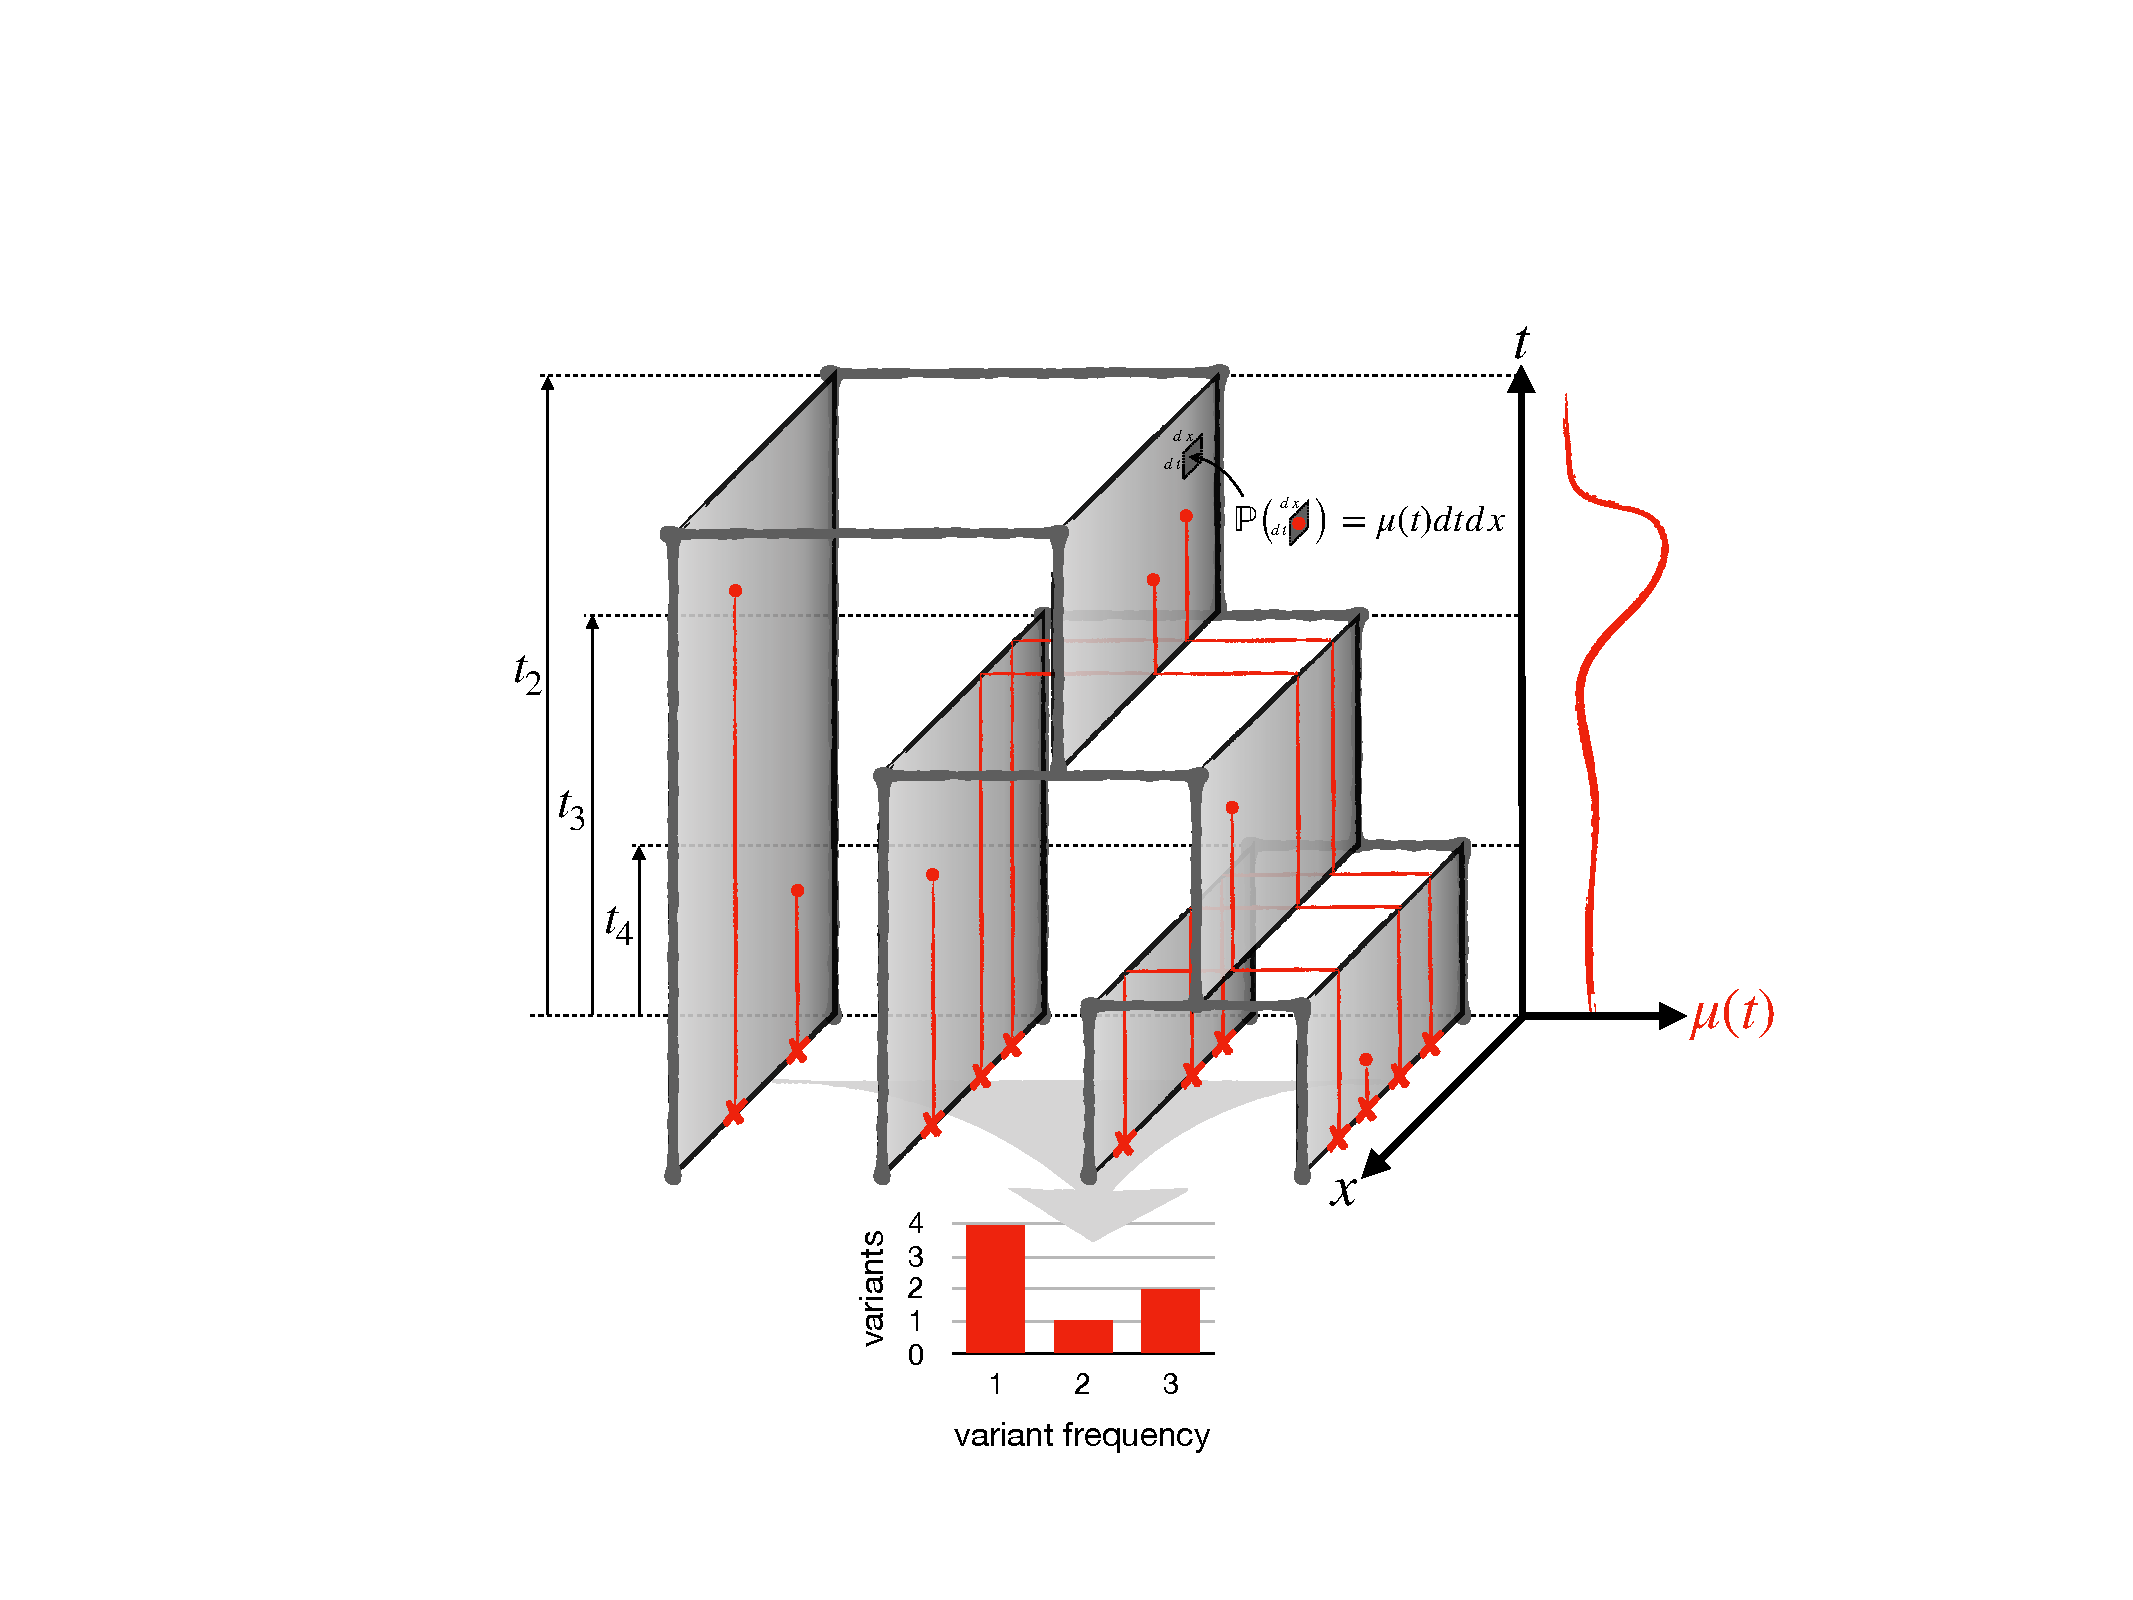
\includegraphics[width=\textwidth]{figures/model}
\caption{Schematic of the marked Poisson process model with $n=4$.
We condition on coalescent times $T_4=t_4,T_3=t_3,T_2=t_2$ and consider mutation intensity function $\mu(t)$.
Red dots indicate mutation events placed by time $t$, genomic position $x$, and coalescent line (which are depicted as extruded in the genomic coordinate axis, grey sheets).
The probability that a differential element $dxdt$ on a given sheet contains a mutation is proportional to the instantaneous mutation intensity $\mu(t)$.
}
\label{fig:model}
\end{figure}

For numerical implementation we consider finite-dimensional approximations of $\eta(t)$ and $\mu(t)$ as piecewise constant on $m$ common epochs $[t_0, t_1), [t_1, t_2),\dots, [t_{m-1}, t_m)$ where $0=t_0 < t_1 < \dots < t_{m-1} < t_m=\infty$.
We take the epoch boundaries as fixed parameters, and in practice make them dense so as to approximate infinite-dimensional histories.
Let $\boldsymbol y = (y_1,\dots,y_m)$ denote the constant population size $\eta(t)$ during each epoch, and let $\boldsymbol z = (z_1,\dots,z_m)$ denote the constant mutation intensity $\mu(t)$ during each epoch.
In Appendix \ref{sec:appendix:pcsws} we show the linear transform \eqref{eqn:transform} reduces to the matrix equation
\begin{equation}
\label{eqn:transform_discrete}
\boldsymbol \xi = L_{n, \boldsymbol y} \boldsymbol z,
\end{equation}
where the $(n-1)\times m$ matrix $L_{n, \boldsymbol y}$ is fixed given a fixed demographic history $\boldsymbol y$.

In linkage equilibrium the log likelihood function of the mutation intensity history $\boldsymbol z$ given an observed SFS vector $\boldsymbol x = (x_1,\dots,x_{n-1})$ and demographic history $\boldsymbol y$ is given by the Poisson random field approximation \citep{}
\[
\ell(\boldsymbol z; \boldsymbol x, \boldsymbol y, n) = \boldsymbol x^\intercal\log(L_{n, \boldsymbol y} \boldsymbol z) - \boldsymbol 1^\intercal L_{n, \boldsymbol y} \boldsymbol z,
\]
where $\log(\cdot)$ operates elementwise, and we've dropped a constant term wrt $\boldsymbol z$.

%WD more inverse problem intro
The inverse problem \eqref{eqn:transform} is ill-posed in general, so many very different histories can be equally consistent with the data \citep{oscillation paper? Yun's other papers?}.
In order to recover smooth histories,
we penalize the $L^p$ norms
of the derivative of $\mu$
\[
\left\| \frac{d \mu}{d t} \right\|_p^p
= \int_0^\infty\left|\frac{d\mu(t)}{dt}\right|^p dt,
\]
for $p=1$ and 2.
With time discretized \eqref{eqn:transform_discrete},
this becomes
\[
\left\|\Delta\boldsymbol z \right\|_p^p.
\]
where $\Delta$ denotes the first difference matrix.
Our cost function (penalized log-likelihood) is then
\begin{equation}
\label{eqn:penalized}
C(\bm z)
%\tilde\ell(\boldsymbol z)
= -\ell(\boldsymbol z) + \lambda \left(\alpha\left\|\Delta\boldsymbol z\right\|_1 + \frac{(1-\alpha)}{2}\left\|\Delta\boldsymbol z\right\|_2^2\right),
\end{equation}
where $\lambda$ tunes the regularization strength, and $\alpha$ tunes the relative $p=1$ vs $p=2$ regularization.
\textcolor{blue}{Kam note: probably we need a ``Ridge'' (Tikhonov)
term like the following to deal with small singular values:}
\[
\lambda' \| \bm z \|_2^2
\]


\section*{Results}\label{sec:results}

% Todo:
% \begin{itemize}
% \item repeat 1KG analysis like in \cite{Harris2017-fw}, see if we recapitulate Kelley's simulation-based pulse results
% \item cluster triplet time series to see if we pull in minor components.
% \end{itemize}

\begin{figure}
  \centering
  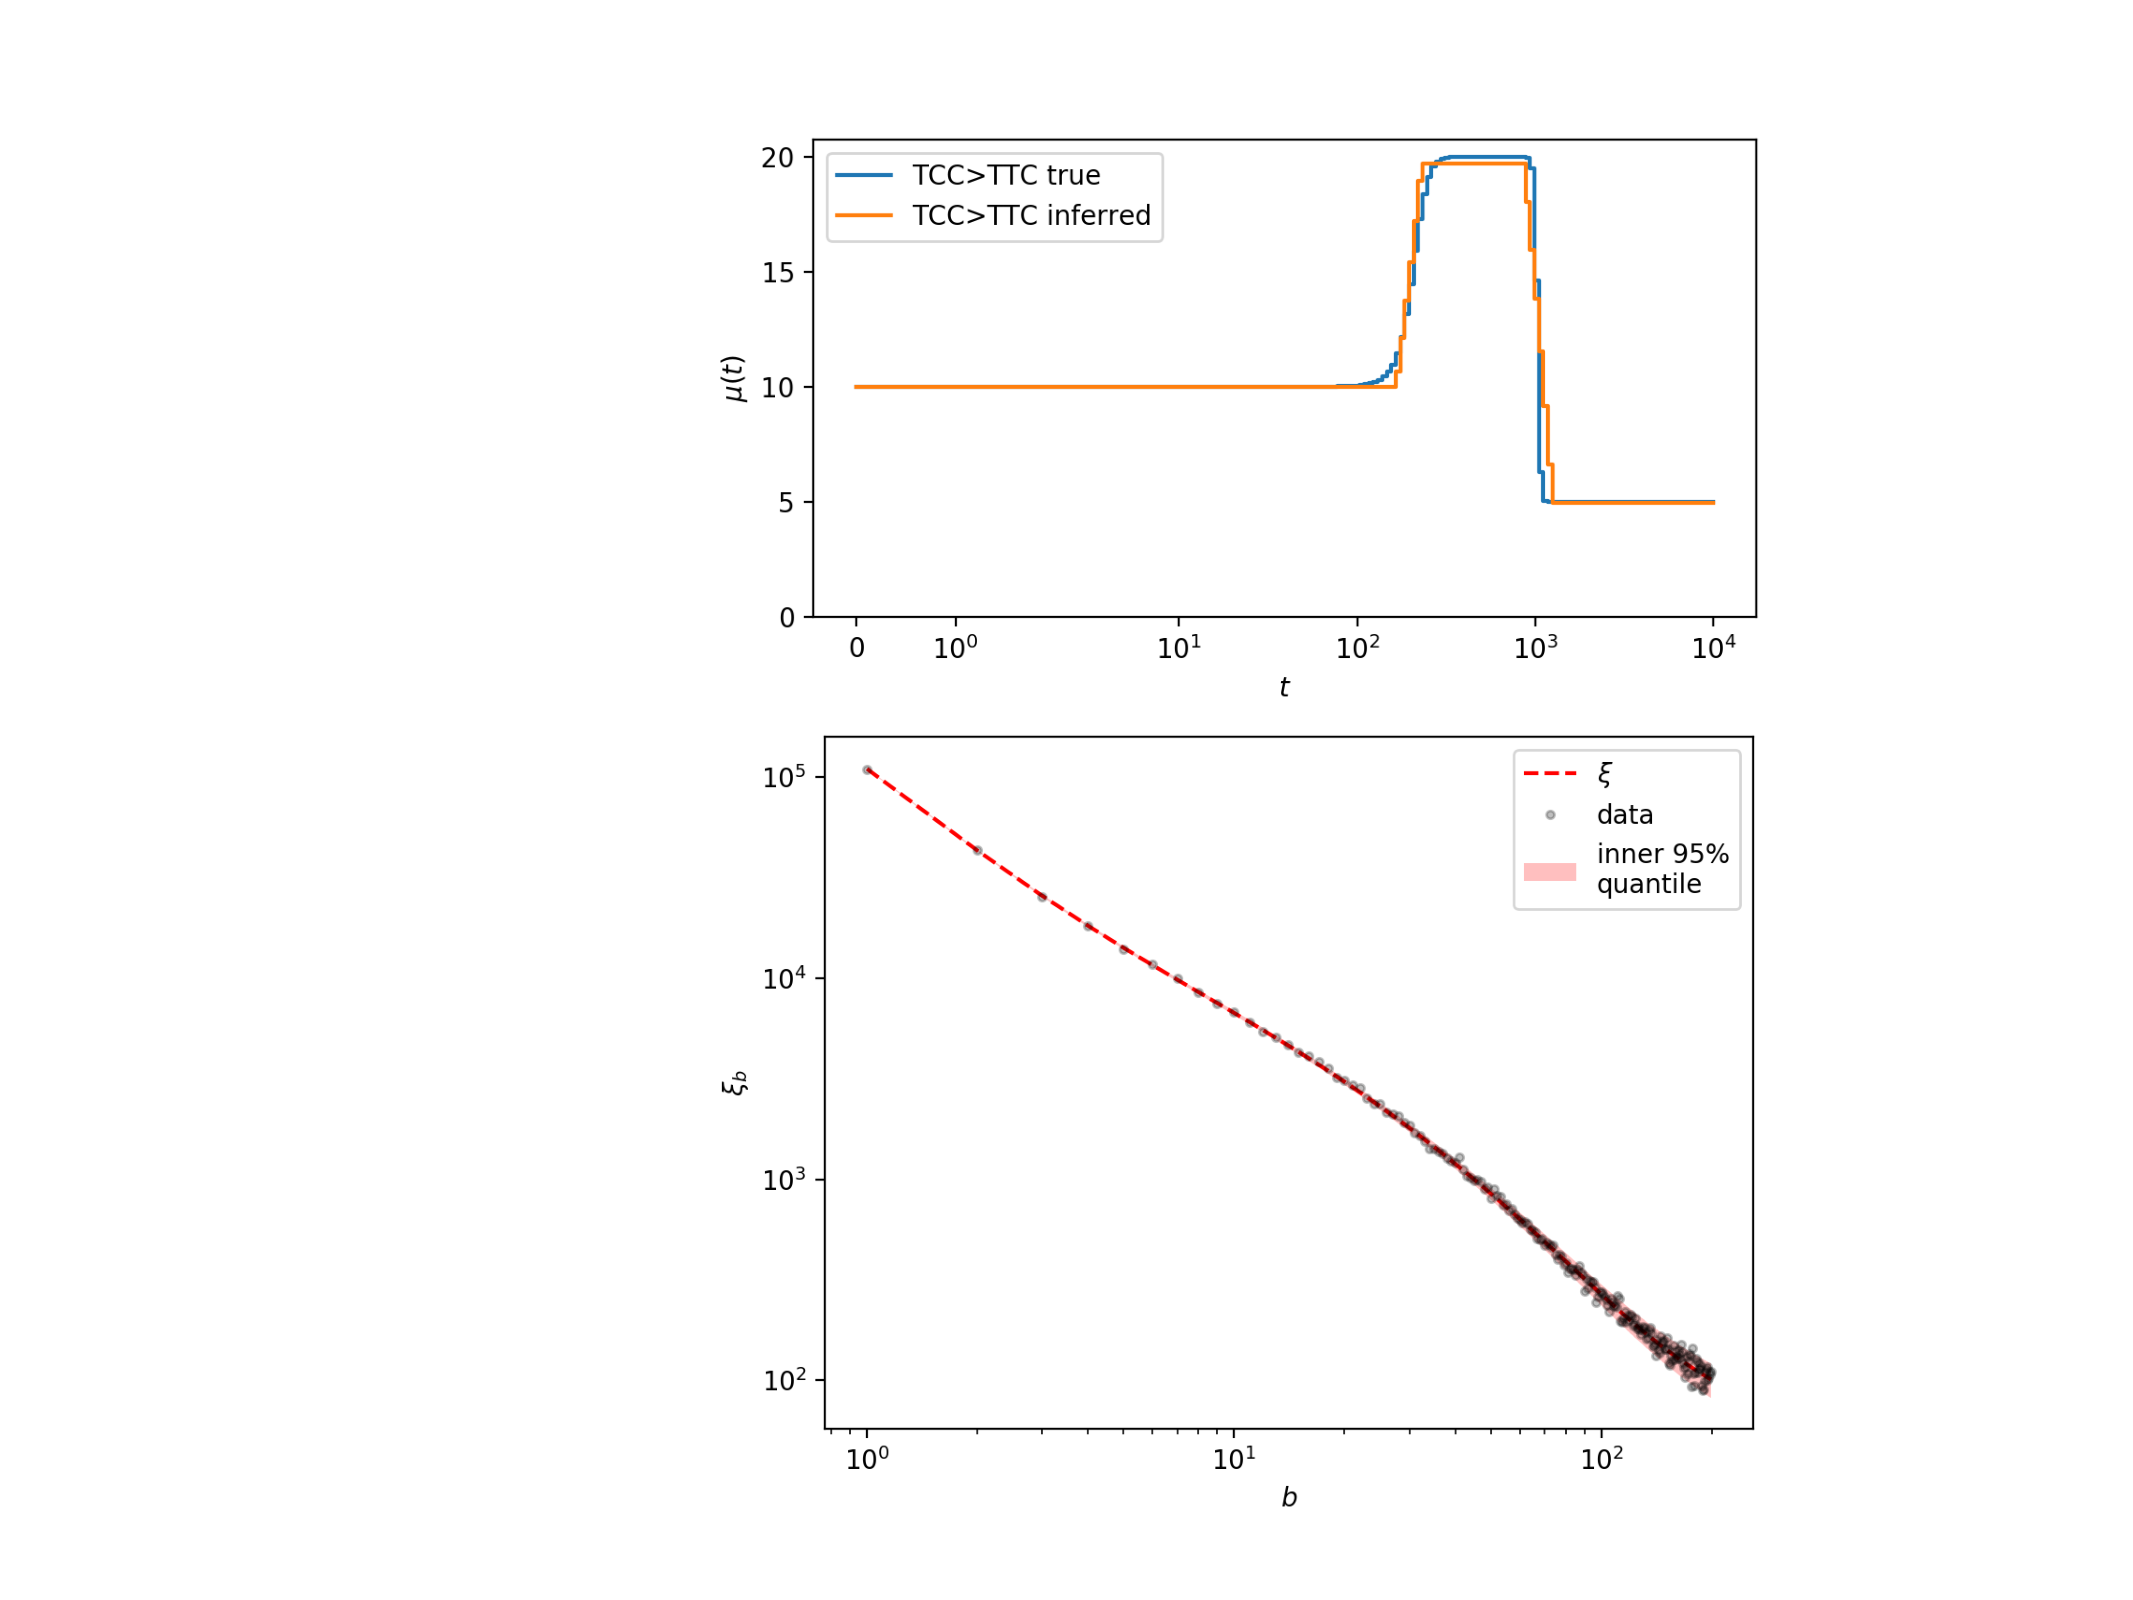
\includegraphics[width=.7\textwidth]{figures/fit_teaser}
  \caption{Simulating and inverting a pulse.}
  \label{}
\end{figure}

\subsection*{Tempora incognita: observability toward the coalescent horizon}\label{sec:model:loss}

Todo: SVD on $L_{n, \boldsymbol y}$

Intuitively, we know the SFS can't contain any information about the history beyond the TMRCA $T_2$, since mutations that occurred before then will not be segregating in the sample.
Thus, we will find it useful to penalize complexity in the history more heavily at times that are more probably ancestral to the TMRCA.

From \eqref{eqn:pi} and \eqref{eqn:r} in the Appendix \ref{sec:appendix}, the CDF of $T_2$ is
\begin{align}
F_2(t) &= 1 - \sum_{j=2}^n A_{2,j}r_2(t)\\
&= 1 - \sum_{j=2}^n A_{2,j}r_2(t)
\end{align}


\section*{Discussion}\label{sec:discussion}

Joint inference of $\eta$ and $\mu$.


\section*{Methods}\label{sec:methods}

\subsection*{Implementation and pipeline}\label{sec:methods:tool}

The \texttt{mushi} software package is available at \url{https://github.com/harrispopgen/mushi}.
%WD cite whatever packages we use, e.g. proxtv, msprime, stdpopsim, etc.

\section*{Acknowledgements}\label{sec:ack}

\bibliographystyle{plainnat}
\bibliography{refs}


\appendix
\section{Appendix}\label{sec:appendix}

\subsection{The expected SFS given demographic and mutation intensity histories}\label{sec:appendix:xi}

Suppose $n$ haplotypes are sampled in the present, and let rvs $(T = T_2,\dots,T_n)$ denote the coalescent times measured retrospectively from the present (i.e. $T_n$ is the most recent coalescent time, and $T_2$ is the TMRCA of the sample).
As in \cite{Griffiths1998-qf} \S3, we consider a marked Poisson process in which every mutation is assigned a random label drawn iid from the uniform distribution on $(0,1)$.
This is tantamount to the infinite sites assumption, with the unit interval representing the genome, and the random variate labels representing mutant sites.
%WD Kam suggests replacing below with $\mu^* \ge \mu(t) \ge 0$, but I don't get why
Further suppose that mutation intensity is not constant, but a specified function of time $0\le \mu(t)<\infty$ (measured in mutations per genome per generation) applying equally to all lines in the coalescent tree at a given time $t$ (measured retrospectively from the present in units of Wright-Fisher generations).
A given line in the coalescent tree then acquires mutations on a genomic subinterval $(x,x+\delta x)$ at rate $\mu(t)\delta x$.
The following argument can be generalized to allow the labelling distribution to be nonuniform over the unit interval, but the same results follow.

Let rv $\mathcal{E}_{\delta x, b}$ denote the event that a mutation present in $b\in\{1, 2, \dots, n-1\}$ haplotypes in the sample occurred within a given genomic interval $(x,x+\delta x)$ (the probability of this event is independent of $x$, given the uniform labeling distribution).
Let $I_k$ denote the $k$th intercoalescent time interval, i.e.\ $I_n = (0, T_n),\ I_{n-1} = (T_n, T_{n-1}),\ \dots,\ I_2 = (T_3, T_2)$.
Let rv $\mathcal{E}_{\delta x, b, k}$ denote the event that the mutation $\mathcal{E}_{\delta x, b}$ occurred during $I_k$.
For small $\delta x$ and finite $\mu(t)$ we have
\begin{align*}
\mathbbm{P}(\mathcal{E}_{\delta x, b}\mid T) &= \sum_{k=2}^n \mathbbm{P}(\mathcal{E}_{\delta x, b, k}\mid T)\\
&= \sum_{k=2}^n p_{n,k}(b)\left(k\delta x\int_{t\in I_k}\mu(t)dt + O((\delta x)^2)\right),
\end{align*}
where
\begin{equation}
\label{eqn:p}
p_{n,k}(b) = \frac{\binom{n-b-1}{k-2}}{\binom{n-1}{k-1}}
\end{equation}
is the probability that a mutant that arose when there were $k$ ancestral lines of $n$ sampled haplotypes will be present in $b$ of them (see \cite{Griffiths1998-qf} eqn 1.9), and the quantity in parentheses is the probability that a mutation arose during the $k$th intercoalescent interval in a small genomic interval of size $\delta x$.
Marginalizing $T$ gives
\begin{align*}
\mathbbm{P}(\mathcal{E}_{\delta x, b}) &= \delta x\sum_{k=2}^n k p_{n,k}(b) \mathbbm{E}_T\left[\int_{t\in I_k}\mu(t)dt\right] + O((\delta x)^2).
\end{align*}
For small $\delta x$, each such interval contains zero or one mutations, so the expected number of mutations subtending $b$ haplotypes (i.e.\ the $b$th component of the SFS) is
\[
\xi_b = \int_0^1 \mathbbm{P}(\mathcal{E}_{dx, b})dx = \sum_{k=2}^n k p_{n,k}(b)\mathbbm{E}_T\left[\int_{t\in I_k}\mu(t)dt\right]\nonumber
\]
Using the explicit bounds of the intercoalescent intervals, $I_{k} = (T_{k+1}, T_k)$, gives
\begin{align}
\label{eqn:xi}
\xi_b &= \sum_{k=2}^n k p_{n,k}(b) \mathbbm{E}_{T_k}\left[\int_0^{T_k}\mu(t)dt\right] - \sum_{k=2}^{n-1} k p_{n,k}(b) \mathbbm{E}_{T_{k+1}}\left[\int_0^{T_{k+1}}\mu(t)dt\right]\nonumber\\
&= \sum_{k=2}^n k p_{n,k}(b) \mathbbm{E}_{T_k}\left[\int_0^{T_k}\mu(t)dt\right] - \sum_{k=3}^{n} (k-1) p_{n,k-1}(b) \mathbbm{E}_{T_{k}}\left[\int_0^{T_k}\mu(t)dt\right]\nonumber\\
&= \sum_{k=2}^n B_{b,k} \mathbbm{E}_{T_k}\left[\int_0^{T_k}\mu(t)dt\right],
\end{align}
where
\begin{equation}
\label{eqn:B}
B_{b,k}\equiv
\begin{cases}
k p_{n,k}(b),& k=2\\
k p_{n,k}(b) - (k-1) p_{n,k-1}(b),& k > 2
\end{cases}
\end{equation}

\cite{Polanski2003-kg} (eqns 5-8) give the marginal density for the coalescent time $T_k$ as
\begin{equation}
\label{eqn:pi}
\pi_k(t_k) = \sum_{j=k}^n A_{k,j} q_j(t_k)
\end{equation}
where
\begin{align*}
A_{k,j} &\equiv \frac{\prod_{l=k\ne j}^{n}\binom{l}{2}}{\prod_{l=k\ne j}^{n}\left[\binom{l}{2}-\binom{j}{2}\right]}, k\le j\le n,\\
A_{n,n} &\equiv 1,\\
q_j(t) &\equiv \frac{\binom{j}{2}}{\eta(t)}\exp\left[-\binom{j}{2}\int_0^t\frac{dx}{\eta(x)}\right],
\end{align*}
and $\eta(t)$ is the haploid effective population size history.
Note that $q_j(t)$ is the density of the time to the first coalescent event among any subset of $j$ individuals in the present, with inhomogeneous Poisson intensity function $\binom{j}{2}/\eta(t)$.

The expectations in \eqref{eqn:xi} can be expressed using \eqref{eqn:pi} as
\begin{align}
\label{eqn:exp}
\mathbbm{E}_{T_k}\left[\int_0^{T_k}\mu(t)dt\right] &= \int_0^\infty\pi_k(t_k)\int_0^{t_k}\mu(t)dt dt_k\nonumber\\
&= \sum_{j=k}^n A_{k,j}\int_0^\infty q_j(t_k)\int_0^{t_k}\mu(t)dt dt_k\nonumber\\
&= \sum_{j=k}^n A_{k,j}\int_0^\infty q_j(t_k)\int_0^\infty 1_{[0<t<t_k]}(t)\mu(t)dt dt_k\nonumber\\
&= \sum_{j=k}^n A_{k,j}\int_0^\infty r_j(t)\mu(t)dt
\end{align}
where in the last line we've exchanged integration order and defined the inhomogeneous Poisson survival function
\begin{equation}
\label{eqn:r}
r_j(t) \equiv \exp\left[-\binom{j}{2}\int_0^t\frac{dx}{\eta(x)}\right]
\end{equation}
corresponding to density $q_j(t)$ (that this is the appropriate survival function can be seen by considering the limit of a sequence of Bernoulli failures).

Using \eqref{eqn:exp} in \eqref{eqn:xi} gives
\begin{align}
\label{eqn:xi2}
\xi_b &= \sum_{k=2}^n B_{b,k} \sum_{j=k}^n A_{k,j}\int_0^\infty r_j(t)\mu(t)dt\nonumber\\
&= \sum_{j=2}^n \left(\sum_{k=2}^j B_{b,k} A_{k,j}\right) \int_0^\infty r_j(t)\mu(t)dt,
\end{align}
where we've exchanged summation order in the last line.

We then have a linear expression for the expected SFS as a function of the mutation intensity history $\mu(t)$:
\begin{equation}
\label{eqn:xivec}
\boldsymbol\xi = C \boldsymbol d,
\end{equation}
where the $(n-1)\times(n-1)$ matrix
\[
C_{b,j} \equiv \sum_{k=2}^j B_{b,k} A_{k,j}
\]
is constant wrt $\mu$ \emph{and} $\eta$, and
\begin{equation}
\label{eqn:d}
d_j \equiv \int_0^\infty r_j(t)\mu(t)dt = \int_0^\infty \exp\left[-\binom{j}{2}\int_0^t\frac{dx}{\eta(x)}\right]\mu(t)dt
\end{equation}
is a linear functional of $\mu$ and a nonlinear functional of $\eta$.
We recover \ref{eqn:transform} by defining the operator $\mathcal{L}_{n,\eta}$ such that $\left(\mathcal{L}_{n,\eta}\mu\right)_j \equiv C \int_0^\infty \exp\left[-\binom{j}{2}\int_0^t\frac{dx}{\eta(x)}\right]\mu(t)dt$.

\subsection{Computing the elements of $C$}\label{sec:appendix:C}

%WD Kam suggests just doing C = B A, but computing the elements of B and A would seem computationally infeasible
We next develop an efficient recursive procedure for computing the $(n-1)\times(n-1)$ matrix $C$.
Using \eqref{eqn:B}
\begin{align*}
C_{b,j} &= \sum_{k=2}^j k p_{n,k}(b) A_{k,j} - \sum_{k=3}^j (k-1) p_{n,k-1}(b) A_{k,j}\\
&= W_{b,j}^{(1)} - W_{b,j}^{(2)},
\end{align*}
where
\begin{align}
\label{eqn:W1}
W_{b,j}^{(1)} &\equiv \sum_{k=2}^j k p_{n,k}(b) A_{k,j}\\
\label{eqn:W2}
W_{b,j}^{(2)} &\equiv \sum_{k=3}^j (k-1) p_{n,k-1}(b) A_{k,j}.
\end{align}
\cite{Polanski2003-ll} (eqn 11) show that $A$ can be expressed as
\[
A_{k,j} = \frac{n! (n-1)!}{(j+n-1)! (n-j)!} \frac{(2 j-1)}{j (j-1)} \frac{(j+k-2)!}{ (k-1)! (k-2)! (j-k)! }(-1)^{j-k},
\]
so, given the form of $p_{n,k}(b)$ in \ref{eqn:p} it's clear that \eqref{eqn:W1} and \eqref{eqn:W2} are definite sums over geometric terms.
Zeilberger's algorithm, which finds polynomial recurrences for definite sums of hypergeometric terms \cite{petkovvsek1996b, paule1995mathematica}, can thus be used to yield the following procedurally generated second-order recursions in $j$:
%WD need to wrap this eqn, as it runs will beyond the margin. Also make an appendix at some point for these
\begin{align*}
&W_{b,2}^{(1)} = \frac{6}{(n+1)}\\
&W_{b,3}^{(1)} = \frac{10(5n-6b-4)}{(n+2)(n+1)}\\
&W_{b,j+2}^{(1)} = -\frac{(2 j+3) \left(-(2 j-1) W_{b,j+1}^{(1)}  \left(2 j (j+1) \left(b^2 \left(j^2+j-2\right)-6 b-j (j+1)-2\right)-j (j+1) n \left(3 b \left(j^2+j+2\right)+j^2+j-2\right)+\left(j (j+1) \left(j^2+j+6\right)+4\right) n^2+4 n\right)-(j-1) (j+1)^2 (j-n) W_{b,j}^{(1)}  (4 (n+1)-j (j+2) (b-n-1))\right)}{j^2 (j+2) (2 j-1) (j+n+1) \left(-b j^2+b+\left(j^2+3\right) (n+1)\right)}
\end{align*}
and
\begin{align*}
&W_{b,2}^{(2)} = 0\\
&W_{b,3}^{(2)} = \frac{20 (n-2)}{(n+1)(n+2)}\\
&W_{b,j+2}^{(2)} = \frac{(2 j+3) (j-n+1)}{j} \left(\frac{(j+1)}{(2 j-1) (j+n)}W_{b,j}^{(2)}-\frac{(j (j+1) (2 b-n+1)-2 (n+1))}{(j-1) (j+2) (j-n) (j+n+1)}W_{b,j+1}^{(2)}\right)
\end{align*}
This completes the framing of mutation intensity inference as a linear inverse problem.

\subsection{Finite-dimensional parameterization of $\eta(t)$ and $\mu(t)$}\label{sec:appendix:pcsws}

%WD Kam describes this discretization as ad hoc, but I'm pretty sure this is your textbook Riemann sum with rectangular partitions. We could do fancier quadrature, but then we'll be less able to lean on previous work (i.e. Rosen et al.)

Following \cite{Rosen2018-bb} (appendix proof of Prop.\ (1)) let $R_\eta(t) \equiv \int_0^t\frac{dx}{\eta(x)}$, and substitute $\tau \equiv R_\eta(t)$ in \eqref{eqn:d} to give
\begin{equation}
\label{eqn:d2}
d_j = \int_0^\infty \exp\left[-\binom{j}{2}\tau\right] \tilde\eta(\tau)\tilde\mu(\tau)d\tau,
\end{equation}
where $\tilde\eta(\tau) \equiv \eta(R^{-1}(\tau))$ and $\tilde\mu(\tau) \equiv \mu(R^{-1}(\tau))$.
We consider piecewise constant $\eta$ and $\mu$ on $m$ common epochs $[t_0, t_1), [t_1, t_2),\dots, [t_{m-1}, t_m)$ where $0=t_0 < t_1 < \dots < t_{m-1} < t_m=\infty$ (not to be confused with the coalescent time realizations in section \ref{sec:appendix:xi}).
We take the epochs as fixed parameters, and in practice make them dense so as to approximate infinite-dimensional histories.
Let $(y_1,\dots,y_m)$ denote the constant population size $\eta(t)$ during each epoch, and let $(z_1,\dots,z_m)$ denote the constant mutation intensity $\mu(t)$ during each epoch.
Let $u_l \equiv \exp(-(t_l-t_{l-1})/y_l)$ for $l=1,\dots,m$. %, and $u_0\equiv 1$.
%WD Kam hates the latin loooooooool. It really does follow by dropping in the y vector and proceeding as in their proof
With this we can follow the proof of Prop.\ (1) in \cite{Rosen2018-bb} mutatis mutandis to arrive at
\begin{equation}
\label{eqn:d3}
\boldsymbol d = M(\boldsymbol y) \boldsymbol z
\end{equation}
where
\begin{equation}
\label{eqn:M}
M(\boldsymbol y) \equiv
\begin{bmatrix}
1 &             &        &                       \\
  & \frac{1}{3} &        &                       \\
  &             & \ddots &                       \\
  &             &        & \frac{1}{\binom{n}{2}}
\end{bmatrix}
\begin{bmatrix}
1       & u_1                & \hdots & \prod_{i=1}^{m-1}u_i               \\
1       & u_1^3              & \hdots & \prod_{i=1}^{m-1}u_i^3             \\
\vdots  & \vdots             & \ddots & \vdots                                \\
1       & u_1^{\binom{n}{2}} & \hdots & \prod_{i=1}^{m-1}u_i^{\binom{n}{2}}
\end{bmatrix}
\begin{bmatrix}
1  &      &        &             &       \\
-1 & 1  &        &             &       \\
     & -1 & 1    &             &       \\
     &      & \ddots & \ddots      &       \\
     &      &        & -1 & 1
\end{bmatrix}
\begin{bmatrix}
y_1 &     &      &             &       \\
    & y_2 &      &             &       \\
     &     & y_3 &             &       \\
     &      &    & \ddots      &       \\
     &      &        &  & y_m
\end{bmatrix}.
\end{equation}
Note that the $(n-1)\times m$ matrix $M(\boldsymbol y)$ is a nonlinear function of the demographic history $\boldsymbol y$ because the $u_l$ are nonlinear functions of $\boldsymbol y$.

Combining \ref{eqn:d3} with \ref{eqn:xivec} gives the discretized inverse problem
\begin{equation}
\boldsymbol\xi = C M(\boldsymbol y) \boldsymbol z = L_{n, \boldsymbol y} \boldsymbol z,
\end{equation}
where $L_{n, \boldsymbol y}\equiv C M(\boldsymbol y)$.



\end{document}
